\documentclass[pdf]{beamer}

\usepackage[utf8]{inputenc}
\usepackage[brazil]{babel}
\usepackage{graphicx}
\usepackage[normalem]{ulem}
\usepackage{listings}
\usepackage{hyperref}

\hypersetup{colorlinks=true,linkcolor=blue,urlcolor=blue,citecolor=blue,anchorcolor=blue}

\lstset{breakatwhitespace,
  language=C,
  columns=fullflexible,
  keepspaces,
  breaklines,
  tabsize=4,
  showstringspaces=false,
  extendedchars=true,
  keywordstyle=\color{blue}\ttfamily,
  stringstyle=\color{red}\ttfamily,
  commentstyle=\color{green!40!black}\ttfamily,
  morecomment=[l][\color{magenta}]{\#}
}

\lstset{breakatwhitespace,
  language=Python,
  columns=fullflexible,
  keepspaces,
  breaklines,
  tabsize=4,
  showstringspaces=false,
  extendedchars=true,
  keywordstyle=\color{blue}\ttfamily,
  stringstyle=\color{red}\ttfamily,
  commentstyle=\color{green!40!black}\ttfamily,
  morecomment=[l][\color{magenta}]{\#}
}

\usetheme{progressbar}

\title[PyUSB]{Easy USB device access}
\subtitle{with PyUSB}

\author{{\Large Wander Lairson Costa}}
\institute{{\large Mozilla Corporation}}

\date{}

\begin{document}

\begin{frame}
  \titlepage
  \begin{center}
    \begin{tabular}{c}
      \url{https://twitter.com/walac00} \\
      \url{https://github.com/walac} \\
      \url{https://br.linkedin.com/in/walac} \\
    \end{tabular}
  \end{center}
\end{frame}

\begin{frame}{USB Introduction}
  \begin{center}
    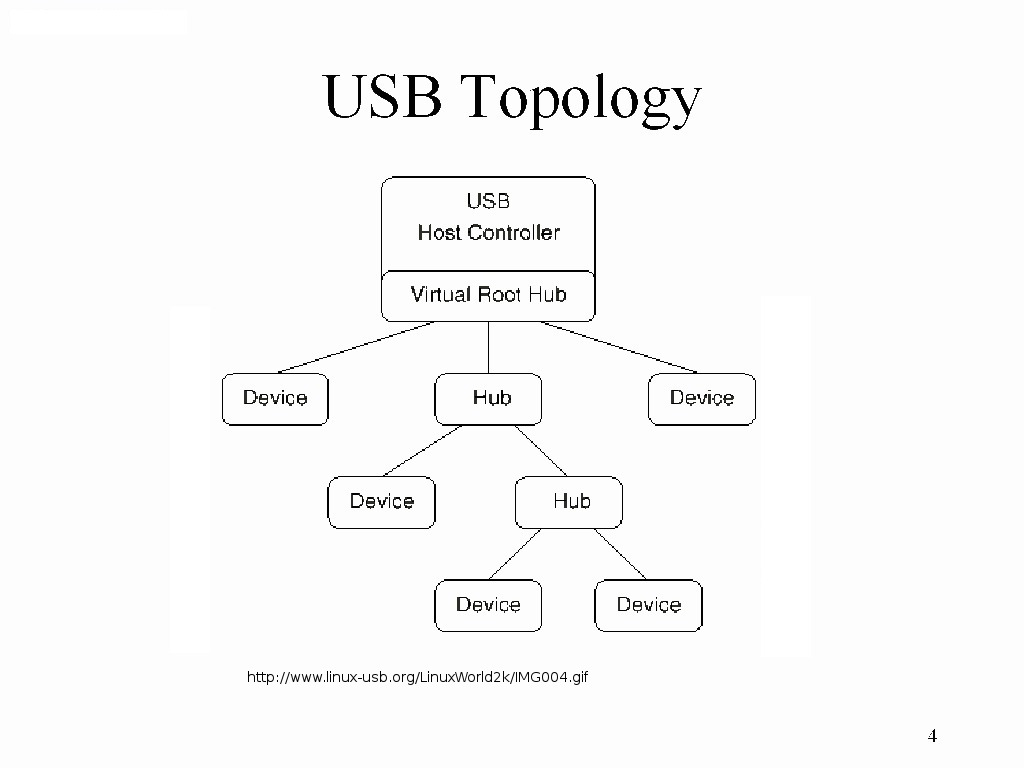
\includegraphics[scale=0.15]{img/topology.jpg}
  \end{center}
  \begin{itemize}
    \tiny
    \item Universal Serial Bus
    \item Created to replace several slow connections (serial, parallel, etc)
    \item It is hot plug and play bus. You don't need to turn off your computer
        connect a new device.
    \item It works as a Master/Slave. All requests are initiated by the Host (polling).
  \end{itemize}
\end{frame}

\begin{frame}{USB Descriptors}
  \begin{center}
    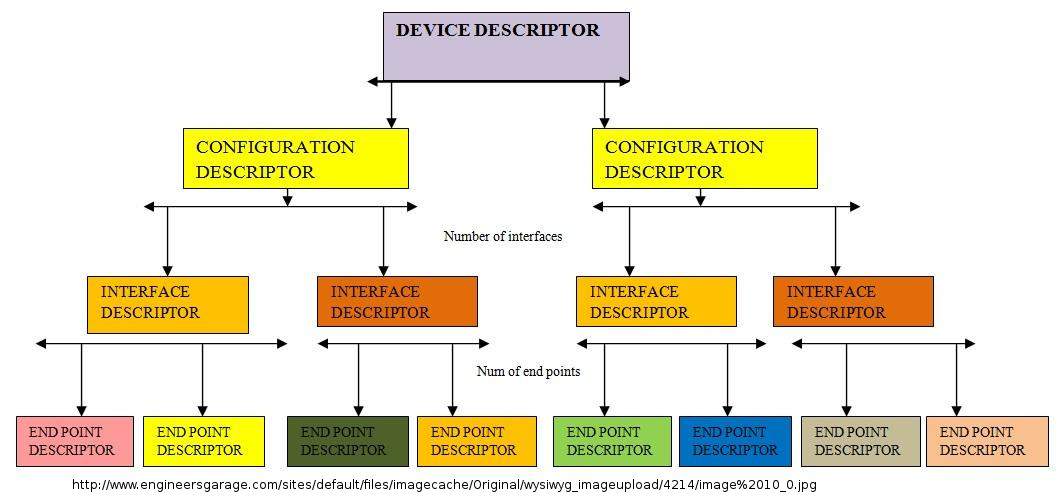
\includegraphics[scale=0.3]{img/descriptors.jpg}
  \end{center}
\end{frame}

\begin{frame}{USB Transfers}
  \begin{center}
    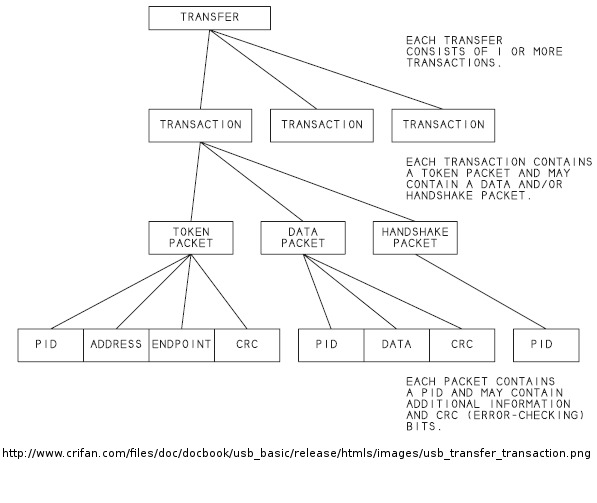
\includegraphics[scale=0.33]{img/usb_transfer.jpg}
  \end{center}
\end{frame}

\begin{frame}{Transfer Types}
  \begin{center}
    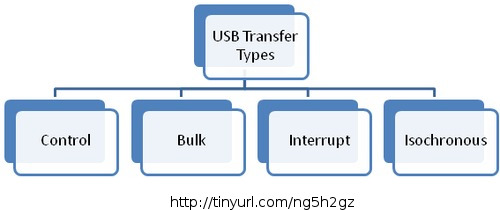
\includegraphics[scale=0.35]{img/transfer_types.jpg}
  \end{center}
  \begin{description}
    \tiny
    \item[Control] used by the Host to configure devices. It is the only transfer
      which supports bidirectional endpoints and which has its format defined by
      the USB spec.
    \item[Bulk] typically used to transfer large amount of data, such as
      printers and disks. The bandwidth allocation can vary, according to the
      bus availability.
    \item[Interrupt] typically used for lower latency, short data transfers. It
      is often used by input devices suchs as mouse and keyboards. Despite its
      name, it works by device polling from the Host.
    \item[Isochronous] used for real time streaming. It prioritizes date rate,
      and it is the only transfer which does not guarantee data delivery, no
      CRC check or retry is performed.
  \end{description}
\end{frame}

\begin{frame}{Accessing USB devices}
  \pause
  Possible solutions:
  \begin{enumerate}
    \pause
    \item Write a kernel device driver.
    \pause
    \item Write a user mode device driver.
    \pause
    \item Use a generic USB library:
      \pause
      \begin{itemize}
          \item libusb 0.1
          \item libusb 1.0
          \item \sout{libusbx}
          \item OpenUSB
          \item libusb-win32
          \item libusbK
      \end{itemize}
      \begin{itemize}
        \pause
        \item Which one to use?
        \pause
        \item PyUSB anwser: anyone!
      \end{itemize}
  \end{enumerate}
\end{frame}

\begin{frame}{PyUSB}
  \begin{itemize}
    \item Up to version 0.4, PyUSB was thin wrapper for libusb 0.1
    \item Starting at version 1.0, PyUSB was redesigned to be a
      platform agnostic, library neutral and easy to use USB access
      package for Python.
    \item PyUSB detaches its API from the backend library used.
    \item You can select the backend you want, but in general PyUSB
      selects the most suitable backend for you.
    \item It works on any Python version $\ge$ 2.4!
    \item 100\% written in Python!
  \end{itemize}
\end{frame}

\begin{frame}[fragile]{Demo: Getting the device serial number (C Version)}
  \tiny
  \pause
  \begin{lstlisting}[language=C]
    #include <libusb.h>
    #include <string.h>

    int main(void)
    {
      libusb_device_handle *handle;
      libusb_device *dev;
      struct libusb_device_descriptor desc;
      int transfered;
      char serial_number[256];

      /* initialized the library */
      libusb_init(NULL);

      /* open the device */
      handle = libusb_open_device_with_vid_pid(NULL, 0x4d8, 0xfa2e);

      /* get the serial number */
      dev = libusb_get_device(handle);
      libusb_get_device_descriptor(dev, &desc);
      libusb_get_string_descriptor_ascii(handle, desc.iSerialNumber, serial_number, 256);
      printf("Serial number = %s\n", serial_number);

      /* cleanup resources */
      libusb_close(handle);
      libusb_exit(NULL);
    }
  \end{lstlisting}
\end{frame}

\begin{frame}[fragile]{Demo: Getting the device serial number (Python version)}
  \small
  \pause
  \begin{lstlisting}[language=Python]
   from usb.core import find
   dev = find(idVendor=0x4d8, idProduct=0xfa2e)
   print(dev.serial_number)
  \end{lstlisting}

  \begin{itemize}
    \small
    \pause
    \item It works with libusb 0.1 and libusb 1.0
    \pause
    \item The \texttt{find} function accepts any device descriptor field
    \pause
    \item \texttt{find} can also return all devices that match the criteria
      (\texttt{find\_all=True} argument).
      \begin{lstlisting}[language=Python]
        devices = find(find_all=True) # all devices
        printers = find(bDeviceClass=7, find_all=True) # all printers
      \end{lstlisting}
  \end{itemize}
\end{frame}

\begin{frame}[fragile]{Demo: Writing data to an endpoint (C version)}
  \tiny
  \pause
  \begin{lstlisting}[language=C]
    #include <libusb.h>
    #include <string.h>

    int main(void)
    {
      libusb_device_handle *handle;
      const char data[] = "test";
      int transfered;

      /* initialized the library */
      libusb_init(NULL);

      /* open the device */
      handle = libusb_open_device_with_vid_pid(NULL, 0x4d8, 0xfa2e);

      /* setup device */
      libusb_set_configuration(handle, 1);
      libusb_claim_interface(handle, 0);

      /* transfer the data */
      libusb_bulk_transfer(handle, 1, data, strlen(data), &transfered, 1000);

      /* cleanup resources */
      libusb_release_interface(handle, 0);
      libusb_close(handle);
      libusb_exit(NULL);
    }
  \end{lstlisting}
\end{frame}

\begin{frame}[fragile]{Demo: Writing data to an endpoint (Python version)}
  \small
  \pause
  \begin{lstlisting}[language=Python]
     from usb.core import find
     dev = find(idVendor=0x4d8, idProduct=0xfa2e)
     dev.set_configuration()
     dev.write(1, "test")
  \end{lstlisting}

  \begin{itemize}
    \small
    \pause
    \item You don't need to know the endpoint type, PyUSB takes care of it!
    \pause
    \item Reading is as easy as writing:
    \begin{lstlisting}[language=Python]
      data = dev.read(0x81, 4) # return an array.array object
    \end{lstlisting}
  \end{itemize}
\end{frame}

\begin{frame}{More info}
  Additional resources:
  \begin{description}
    \item[Project page] \url{https://walac.github.io/pyusb}
    \item[Source code] \url{https://github.com/walac/pyusb}
    \item[Tutorial] \url{https://github.com/walac/pyusb/blob/master/docs/tutorial.rst}
  \end{description}
\end{frame}

\begin{frame}{Thank you!}
  \begin{center}
    
\includegraphics[scale=0.2]{img/questions.jpg}
  \end{center}

  \begin{center}
    \begin{tabular}{c l}
      \textbf{Twitter} & \href{https://twitter.com/walac00}{@walac00} \\
      \textbf{Github} & \url{https://github.com/walac} \\
      \textbf{Blog} & \url{https://walac.github.io} \\
      \textbf{Linkedin} & \url{https://br.linkedin.com/in/walac} \\
    \end{tabular}
  \end{center}

\end{frame}

\end{document}

